\documentclass[12pt,]{article}
\usepackage{lmodern}
\usepackage{amssymb,amsmath}
\usepackage{ifxetex,ifluatex}
\usepackage{fixltx2e} % provides \textsubscript
\ifnum 0\ifxetex 1\fi\ifluatex 1\fi=0 % if pdftex
  \usepackage[T1]{fontenc}
  \usepackage[utf8]{inputenc}
\else % if luatex or xelatex
  \ifxetex
    \usepackage{mathspec}
  \else
    \usepackage{fontspec}
  \fi
  \defaultfontfeatures{Ligatures=TeX,Scale=MatchLowercase}
    \setmainfont[]{Times New Roman}
\fi
% use upquote if available, for straight quotes in verbatim environments
\IfFileExists{upquote.sty}{\usepackage{upquote}}{}
% use microtype if available
\IfFileExists{microtype.sty}{%
\usepackage{microtype}
\UseMicrotypeSet[protrusion]{basicmath} % disable protrusion for tt fonts
}{}
\usepackage[margin=2.54cm]{geometry}
\usepackage{hyperref}
\hypersetup{unicode=true,
            pdftitle={Final Project Yifei Zhang},
            pdfauthor={Yifei Zhang},
            pdfborder={0 0 0},
            breaklinks=true}
\urlstyle{same}  % don't use monospace font for urls
\usepackage{color}
\usepackage{fancyvrb}
\newcommand{\VerbBar}{|}
\newcommand{\VERB}{\Verb[commandchars=\\\{\}]}
\DefineVerbatimEnvironment{Highlighting}{Verbatim}{commandchars=\\\{\}}
% Add ',fontsize=\small' for more characters per line
\usepackage{framed}
\definecolor{shadecolor}{RGB}{248,248,248}
\newenvironment{Shaded}{\begin{snugshade}}{\end{snugshade}}
\newcommand{\KeywordTok}[1]{\textcolor[rgb]{0.13,0.29,0.53}{\textbf{#1}}}
\newcommand{\DataTypeTok}[1]{\textcolor[rgb]{0.13,0.29,0.53}{#1}}
\newcommand{\DecValTok}[1]{\textcolor[rgb]{0.00,0.00,0.81}{#1}}
\newcommand{\BaseNTok}[1]{\textcolor[rgb]{0.00,0.00,0.81}{#1}}
\newcommand{\FloatTok}[1]{\textcolor[rgb]{0.00,0.00,0.81}{#1}}
\newcommand{\ConstantTok}[1]{\textcolor[rgb]{0.00,0.00,0.00}{#1}}
\newcommand{\CharTok}[1]{\textcolor[rgb]{0.31,0.60,0.02}{#1}}
\newcommand{\SpecialCharTok}[1]{\textcolor[rgb]{0.00,0.00,0.00}{#1}}
\newcommand{\StringTok}[1]{\textcolor[rgb]{0.31,0.60,0.02}{#1}}
\newcommand{\VerbatimStringTok}[1]{\textcolor[rgb]{0.31,0.60,0.02}{#1}}
\newcommand{\SpecialStringTok}[1]{\textcolor[rgb]{0.31,0.60,0.02}{#1}}
\newcommand{\ImportTok}[1]{#1}
\newcommand{\CommentTok}[1]{\textcolor[rgb]{0.56,0.35,0.01}{\textit{#1}}}
\newcommand{\DocumentationTok}[1]{\textcolor[rgb]{0.56,0.35,0.01}{\textbf{\textit{#1}}}}
\newcommand{\AnnotationTok}[1]{\textcolor[rgb]{0.56,0.35,0.01}{\textbf{\textit{#1}}}}
\newcommand{\CommentVarTok}[1]{\textcolor[rgb]{0.56,0.35,0.01}{\textbf{\textit{#1}}}}
\newcommand{\OtherTok}[1]{\textcolor[rgb]{0.56,0.35,0.01}{#1}}
\newcommand{\FunctionTok}[1]{\textcolor[rgb]{0.00,0.00,0.00}{#1}}
\newcommand{\VariableTok}[1]{\textcolor[rgb]{0.00,0.00,0.00}{#1}}
\newcommand{\ControlFlowTok}[1]{\textcolor[rgb]{0.13,0.29,0.53}{\textbf{#1}}}
\newcommand{\OperatorTok}[1]{\textcolor[rgb]{0.81,0.36,0.00}{\textbf{#1}}}
\newcommand{\BuiltInTok}[1]{#1}
\newcommand{\ExtensionTok}[1]{#1}
\newcommand{\PreprocessorTok}[1]{\textcolor[rgb]{0.56,0.35,0.01}{\textit{#1}}}
\newcommand{\AttributeTok}[1]{\textcolor[rgb]{0.77,0.63,0.00}{#1}}
\newcommand{\RegionMarkerTok}[1]{#1}
\newcommand{\InformationTok}[1]{\textcolor[rgb]{0.56,0.35,0.01}{\textbf{\textit{#1}}}}
\newcommand{\WarningTok}[1]{\textcolor[rgb]{0.56,0.35,0.01}{\textbf{\textit{#1}}}}
\newcommand{\AlertTok}[1]{\textcolor[rgb]{0.94,0.16,0.16}{#1}}
\newcommand{\ErrorTok}[1]{\textcolor[rgb]{0.64,0.00,0.00}{\textbf{#1}}}
\newcommand{\NormalTok}[1]{#1}
\usepackage{longtable,booktabs}
\usepackage{graphicx,grffile}
\makeatletter
\def\maxwidth{\ifdim\Gin@nat@width>\linewidth\linewidth\else\Gin@nat@width\fi}
\def\maxheight{\ifdim\Gin@nat@height>\textheight\textheight\else\Gin@nat@height\fi}
\makeatother
% Scale images if necessary, so that they will not overflow the page
% margins by default, and it is still possible to overwrite the defaults
% using explicit options in \includegraphics[width, height, ...]{}
\setkeys{Gin}{width=\maxwidth,height=\maxheight,keepaspectratio}
\IfFileExists{parskip.sty}{%
\usepackage{parskip}
}{% else
\setlength{\parindent}{0pt}
\setlength{\parskip}{6pt plus 2pt minus 1pt}
}
\setlength{\emergencystretch}{3em}  % prevent overfull lines
\providecommand{\tightlist}{%
  \setlength{\itemsep}{0pt}\setlength{\parskip}{0pt}}
\setcounter{secnumdepth}{5}
% Redefines (sub)paragraphs to behave more like sections
\ifx\paragraph\undefined\else
\let\oldparagraph\paragraph
\renewcommand{\paragraph}[1]{\oldparagraph{#1}\mbox{}}
\fi
\ifx\subparagraph\undefined\else
\let\oldsubparagraph\subparagraph
\renewcommand{\subparagraph}[1]{\oldsubparagraph{#1}\mbox{}}
\fi

%%% Use protect on footnotes to avoid problems with footnotes in titles
\let\rmarkdownfootnote\footnote%
\def\footnote{\protect\rmarkdownfootnote}

%%% Change title format to be more compact
\usepackage{titling}

% Create subtitle command for use in maketitle
\providecommand{\subtitle}[1]{
  \posttitle{
    \begin{center}\large#1\end{center}
    }
}

\setlength{\droptitle}{-2em}

  \title{Final Project Yifei Zhang}
    \pretitle{\vspace{\droptitle}\centering\huge}
  \posttitle{\par}
  \subtitle{\url{https://github.com/yz470/Final-project-for-Environmental-Data-Analytics.git}}
  \author{Yifei Zhang}
    \preauthor{\centering\large\emph}
  \postauthor{\par}
    \date{}
    \predate{}\postdate{}
  

\begin{document}
\maketitle
\begin{abstract}
This project aims at answering the following research questions: 1. Is
there a trend in PM2.5 concentrations in Shanghai from 2012 to 2017? 2.
What is the spatial pattern of PM2.5 concentration in Beijing, Chengdu,
Guangzhou, Shanghai, and Shenyang in 2017? The U.S. Department of State
Air Quality Dataset is used to answer the research questions. Results
show that from 2012 to 2017, there existed a decreasing trend in PM2.5
concentrations in Shanghai. In addition, pronounced seasonal variation
is observed in PM2.5 concentrations in Shanghai, with the highest
concentrations typically observed in the winter and the lowest
concentrations generally found in the summer. Among the 5 cities,
Beijing and Chengdu showed highest average PM2.5 concentration in 2017,
with the AQI level reaching 158.
\end{abstract}

\newpage

\tableofcontents  \newpage
\listoftables  \newpage
\listoffigures  \newpage

\section{Research Question and
Rationale}\label{research-question-and-rationale}

Air pollution is a severe problem in China. It is often the smoggy air
that occurs to many people when it comes to Beijing, the capital of
China. Among the air pollutants, of particular concern is PM2.5
(particles with an aerodynamic diameter less than 2.5 um). Exposure to
high concentrations of PM2.5 results in risks to the cardiovascular
system, cerebrovascular system and an increase in the probability of
cancer and premature death. In recent years, China's government has
taken serious action against air pollution, but there is still a long
way to go.

Given the increasing public concern in air quality and the efforts of
Chinese government to fight air pollution, I am interested in the actual
outcomes: whether or not there is a decreasing trend in air quality over
the years. In particular, I want to examine the PM2.5 trend in Shanghai
because it is the largest city in China by population, and it is also
where I come from. I will use the The U.S. Department of State air
quality files, which contain the hourly PM2.5 concentrations in 5 cities
in China from 2011 to 2017. With this dataset, my second research
question is to look at the spatial pattern of PM2.5 concentrations in
these 5 cities.

Goals:

\begin{itemize}
\tightlist
\item
  Use Mann-Kendall test to analyze trends in PM2.5 concentrations in
  Shanghai from 2012 to 2017
\item
  Run a Pettitt's Test to check if there are changing points
\item
  Check for seasonality in PM2.5 concentrations.
\item
  Use Seasonal Mann-Kendall test if there is seasonality
\item
  Look at which city has the highest average PM2.5 concentration.
\end{itemize}

\newpage

\section{Dataset Information}\label{dataset-information}

The U.S. Department of State air quality files contain hourly PM2.5 or
data in concentration units from each post, as reported on the
www.stateair.net website. Files include hourly data with the following
file name structure: Site\_Year\_DurationParameter.csv. Filename
examples: Beijing\_2013\_HourlyPM2.5.csv

All files contain the following column headers: Site, Parameter, Date
(LST), Year, Month, Day, Hour, Value, Unit, Duration, QC Name.
Definitions and examples of column headers can be found in the table
below.

The air quality data are measured at the U.S. Embassy in Beijing and at
the Consulates in Chengdu, Guangzhou, Shanghai, and Shenyang.

\begin{longtable}[]{@{}lll@{}}
\caption{Data Structure and definition}\tabularnewline
\toprule
\begin{minipage}[b]{0.14\columnwidth}\raggedright\strut
Term\strut
\end{minipage} & \begin{minipage}[b]{0.60\columnwidth}\raggedright\strut
Definitions\strut
\end{minipage} & \begin{minipage}[b]{0.11\columnwidth}\raggedright\strut
Examples\strut
\end{minipage}\tabularnewline
\midrule
\endfirsthead
\toprule
\begin{minipage}[b]{0.14\columnwidth}\raggedright\strut
Term\strut
\end{minipage} & \begin{minipage}[b]{0.60\columnwidth}\raggedright\strut
Definitions\strut
\end{minipage} & \begin{minipage}[b]{0.11\columnwidth}\raggedright\strut
Examples\strut
\end{minipage}\tabularnewline
\midrule
\endhead
\begin{minipage}[t]{0.14\columnwidth}\raggedright\strut
Site\strut
\end{minipage} & \begin{minipage}[t]{0.60\columnwidth}\raggedright\strut
City or post where the measurements were taken.\strut
\end{minipage} & \begin{minipage}[t]{0.11\columnwidth}\raggedright\strut
Beijing, Shenyang\strut
\end{minipage}\tabularnewline
\begin{minipage}[t]{0.14\columnwidth}\raggedright\strut
Parameter\strut
\end{minipage} & \begin{minipage}[t]{0.60\columnwidth}\raggedright\strut
The air quality pollutant measured.\strut
\end{minipage} & \begin{minipage}[t]{0.11\columnwidth}\raggedright\strut
PM2.5, O3\strut
\end{minipage}\tabularnewline
\begin{minipage}[t]{0.14\columnwidth}\raggedright\strut
Date\strut
\end{minipage} & \begin{minipage}[t]{0.60\columnwidth}\raggedright\strut
The date and hour of the measurement in local standard time (e.g., BJT
-- Beijing Time). The date- time format follows YYYY-MM-DD HH:mm, where
00:00 is midnight, 14:00 is 2:00 p.m., etc.\strut
\end{minipage} & \begin{minipage}[t]{0.11\columnwidth}\raggedright\strut
2013-05-01 00:00\strut
\end{minipage}\tabularnewline
\begin{minipage}[t]{0.14\columnwidth}\raggedright\strut
Year\strut
\end{minipage} & \begin{minipage}[t]{0.60\columnwidth}\raggedright\strut
4 digit year that corresponds to YYYY in Date\strut
\end{minipage} & \begin{minipage}[t]{0.11\columnwidth}\raggedright\strut
2013\strut
\end{minipage}\tabularnewline
\begin{minipage}[t]{0.14\columnwidth}\raggedright\strut
Month\strut
\end{minipage} & \begin{minipage}[t]{0.60\columnwidth}\raggedright\strut
1 or 2 digit month (1 to 12) that corresponds to MM in Date\strut
\end{minipage} & \begin{minipage}[t]{0.11\columnwidth}\raggedright\strut
5, 12\strut
\end{minipage}\tabularnewline
\begin{minipage}[t]{0.14\columnwidth}\raggedright\strut
Day\strut
\end{minipage} & \begin{minipage}[t]{0.60\columnwidth}\raggedright\strut
1 or 2 digit day (1 to 31) that corresponds to DD in Date\strut
\end{minipage} & \begin{minipage}[t]{0.11\columnwidth}\raggedright\strut
1, 31\strut
\end{minipage}\tabularnewline
\begin{minipage}[t]{0.14\columnwidth}\raggedright\strut
Hour\strut
\end{minipage} & \begin{minipage}[t]{0.60\columnwidth}\raggedright\strut
1 or 2 digit hour (0 to 23) that corresponds to HH in Date\strut
\end{minipage} & \begin{minipage}[t]{0.11\columnwidth}\raggedright\strut
0, 18\strut
\end{minipage}\tabularnewline
\begin{minipage}[t]{0.14\columnwidth}\raggedright\strut
Value\strut
\end{minipage} & \begin{minipage}[t]{0.60\columnwidth}\raggedright\strut
The measurement in concentration. Missing values are listed as
-999.\strut
\end{minipage} & \begin{minipage}[t]{0.11\columnwidth}\raggedright\strut
45, 450, -999\strut
\end{minipage}\tabularnewline
\begin{minipage}[t]{0.14\columnwidth}\raggedright\strut
Unit\strut
\end{minipage} & \begin{minipage}[t]{0.60\columnwidth}\raggedright\strut
(ug/m3) for PM2.5\strut
\end{minipage} & \begin{minipage}[t]{0.11\columnwidth}\raggedright\strut
ug/m3\strut
\end{minipage}\tabularnewline
\begin{minipage}[t]{0.14\columnwidth}\raggedright\strut
Duration\strut
\end{minipage} & \begin{minipage}[t]{0.60\columnwidth}\raggedright\strut
1-hour (1 Hr) for PM2.5\strut
\end{minipage} & \begin{minipage}[t]{0.11\columnwidth}\raggedright\strut
1 Hr\strut
\end{minipage}\tabularnewline
\begin{minipage}[t]{0.14\columnwidth}\raggedright\strut
QC Name\strut
\end{minipage} & \begin{minipage}[t]{0.60\columnwidth}\raggedright\strut
The quality control status of the data; either valid or missing
(unavailable). Invalid data are not included in these files.\strut
\end{minipage} & \begin{minipage}[t]{0.11\columnwidth}\raggedright\strut
Valid, Missing\strut
\end{minipage}\tabularnewline
\bottomrule
\end{longtable}

\newpage 

\begin{longtable}[]{@{}ll@{}}
\caption{Embassy and Consulate geographic coordinates.}\tabularnewline
\toprule
Site location & Latitude and Longitude Degrees\tabularnewline
\midrule
\endfirsthead
\toprule
Site location & Latitude and Longitude Degrees\tabularnewline
\midrule
\endhead
Beijing & 39.95, 116.47\tabularnewline
Chengdu & 30.63, 104.07\tabularnewline
Guangzhou & 23.12, 113.32\tabularnewline
Shanghai & 31.21, 121.44\tabularnewline
Shenyang & 41.78, 123.42\tabularnewline
\bottomrule
\end{longtable}

\newpage

\section{Exploratory Data Analysis and
Wrangling}\label{exploratory-data-analysis-and-wrangling}

\begin{Shaded}
\begin{Highlighting}[]
\CommentTok{#Look at the general structure of the data, number of observations, maximum and minimum values, among other things}
\KeywordTok{colnames}\NormalTok{(shanghai_}\DecValTok{2017}\NormalTok{)}
\end{Highlighting}
\end{Shaded}

\begin{verbatim}
##  [1] "Site"       "Parameter"  "Date..LST." "Year"       "Month"     
##  [6] "Day"        "Hour"       "Value"      "Unit"       "Duration"  
## [11] "QC.Name"
\end{verbatim}

\begin{Shaded}
\begin{Highlighting}[]
\KeywordTok{dim}\NormalTok{(shanghai_}\DecValTok{2017}\NormalTok{)}
\end{Highlighting}
\end{Shaded}

\begin{verbatim}
## [1] 4344   11
\end{verbatim}

\begin{Shaded}
\begin{Highlighting}[]
\KeywordTok{head}\NormalTok{(shanghai_}\DecValTok{2017}\NormalTok{)}
\end{Highlighting}
\end{Shaded}

\begin{verbatim}
##       Site Parameter    Date..LST. Year Month Day Hour Value  Unit
## 1 Shanghai     PM2.5 1/1/2017 0:00 2017     1   1    0    42 µg/m³
## 2 Shanghai     PM2.5 1/1/2017 1:00 2017     1   1    1    46 µg/m³
## 3 Shanghai     PM2.5 1/1/2017 2:00 2017     1   1    2    56 µg/m³
## 4 Shanghai     PM2.5 1/1/2017 3:00 2017     1   1    3    49 µg/m³
## 5 Shanghai     PM2.5 1/1/2017 4:00 2017     1   1    4    51 µg/m³
## 6 Shanghai     PM2.5 1/1/2017 5:00 2017     1   1    5    49 µg/m³
##   Duration QC.Name
## 1     1 Hr   Valid
## 2     1 Hr   Valid
## 3     1 Hr   Valid
## 4     1 Hr   Valid
## 5     1 Hr   Valid
## 6     1 Hr   Valid
\end{verbatim}

\begin{Shaded}
\begin{Highlighting}[]
\KeywordTok{str}\NormalTok{(shanghai_}\DecValTok{2017}\NormalTok{)}
\end{Highlighting}
\end{Shaded}

\begin{verbatim}
## 'data.frame':    4344 obs. of  11 variables:
##  $ Site      : Factor w/ 1 level "Shanghai": 1 1 1 1 1 1 1 1 1 1 ...
##  $ Parameter : Factor w/ 1 level "PM2.5": 1 1 1 1 1 1 1 1 1 1 ...
##  $ Date..LST.: Factor w/ 4343 levels "1/1/2017 0:00",..: 1 2 13 18 19 20 21 22 23 24 ...
##  $ Year      : int  2017 2017 2017 2017 2017 2017 2017 2017 2017 2017 ...
##  $ Month     : int  1 1 1 1 1 1 1 1 1 1 ...
##  $ Day       : int  1 1 1 1 1 1 1 1 1 1 ...
##  $ Hour      : int  0 1 2 3 4 5 6 7 8 9 ...
##  $ Value     : int  42 46 56 49 51 49 43 47 52 45 ...
##  $ Unit      : Factor w/ 1 level "µg/m³": 1 1 1 1 1 1 1 1 1 1 ...
##  $ Duration  : Factor w/ 1 level "1 Hr": 1 1 1 1 1 1 1 1 1 1 ...
##  $ QC.Name   : Factor w/ 2 levels "Missing","Valid": 2 2 2 2 2 2 2 2 2 2 ...
\end{verbatim}

\begin{Shaded}
\begin{Highlighting}[]
\KeywordTok{summary}\NormalTok{(shanghai_}\DecValTok{2017}\NormalTok{)}
\end{Highlighting}
\end{Shaded}

\begin{verbatim}
##        Site      Parameter             Date..LST.        Year     
##  Shanghai:4344   PM2.5:4344   3/12/2017 3:00:   2   Min.   :2017  
##                               1/1/2017 0:00 :   1   1st Qu.:2017  
##                               1/1/2017 1:00 :   1   Median :2017  
##                               1/1/2017 10:00:   1   Mean   :2017  
##                               1/1/2017 11:00:   1   3rd Qu.:2017  
##                               1/1/2017 12:00:   1   Max.   :2017  
##                               (Other)       :4337                 
##      Month            Day            Hour           Value        
##  Min.   :1.000   Min.   : 1.0   Min.   : 0.00   Min.   :-999.00  
##  1st Qu.:2.000   1st Qu.: 8.0   1st Qu.: 5.75   1st Qu.:  24.00  
##  Median :4.000   Median :16.0   Median :11.50   Median :  39.00  
##  Mean   :3.508   Mean   :15.6   Mean   :11.50   Mean   :  27.87  
##  3rd Qu.:5.000   3rd Qu.:23.0   3rd Qu.:17.25   3rd Qu.:  59.00  
##  Max.   :6.000   Max.   :31.0   Max.   :23.00   Max.   : 188.00  
##                                                                  
##     Unit      Duration       QC.Name    
##  µg/m³:4344   1 Hr:4344   Missing:  73  
##                           Valid  :4271  
##                                         
##                                         
##                                         
##                                         
## 
\end{verbatim}

\begin{Shaded}
\begin{Highlighting}[]
\KeywordTok{summary}\NormalTok{(shanghai_}\DecValTok{2012}\NormalTok{)}
\end{Highlighting}
\end{Shaded}

\begin{verbatim}
##        Site      Parameter               Date..LST.        Year     
##  Shanghai:8784   PM2.5:8784   2012-03-11 03:00:   2   Min.   :2012  
##                               2012-01-01 00:00:   1   1st Qu.:2012  
##                               2012-01-01 01:00:   1   Median :2012  
##                               2012-01-01 02:00:   1   Mean   :2012  
##                               2012-01-01 03:00:   1   3rd Qu.:2012  
##                               2012-01-01 04:00:   1   Max.   :2012  
##                               (Other)         :8777                 
##      Month             Day             Hour           Value        
##  Min.   : 1.000   Min.   : 1.00   Min.   : 0.00   Min.   :-999.00  
##  1st Qu.: 4.000   1st Qu.: 8.00   1st Qu.: 5.75   1st Qu.:  23.00  
##  Median : 7.000   Median :16.00   Median :11.50   Median :  40.00  
##  Mean   : 6.514   Mean   :15.76   Mean   :11.50   Mean   :  17.21  
##  3rd Qu.:10.000   3rd Qu.:23.00   3rd Qu.:17.25   3rd Qu.:  65.00  
##  Max.   :12.000   Max.   :31.00   Max.   :23.00   Max.   : 650.00  
##                                                                    
##     Unit      Duration       QC.Name    
##  µg/m³:8784   1 Hr:8784   Missing:   5  
##                           Valid  :8779  
##                                         
##                                         
##                                         
##                                         
## 
\end{verbatim}

\begin{figure}
\centering
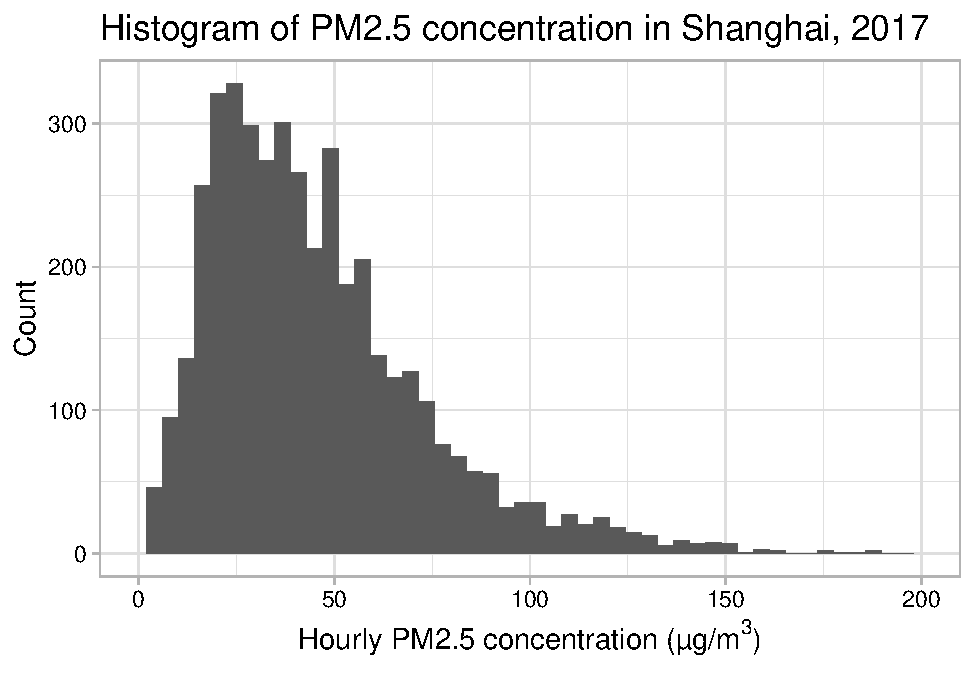
\includegraphics{Project_Template_files/figure-latex/Exploratory graph 1-1.pdf}
\caption{Histogram of PM2.5 concentration in Shanghai, 2017}
\end{figure}

\emph{Figure 1 shows how PM2.5 concentrations spread over the range of
values}

\begin{figure}
\centering
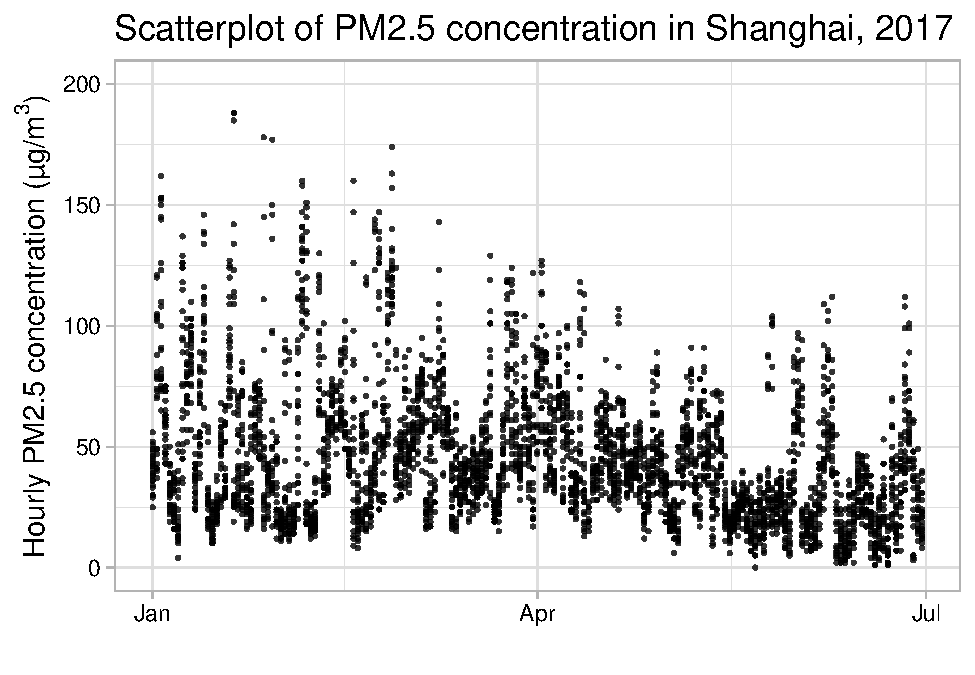
\includegraphics{Project_Template_files/figure-latex/Exploratory graph 2-1.pdf}
\caption{Scatterplot of PM2.5 concentration in Shanghai, 2017}
\end{figure}

\begin{figure}
\centering
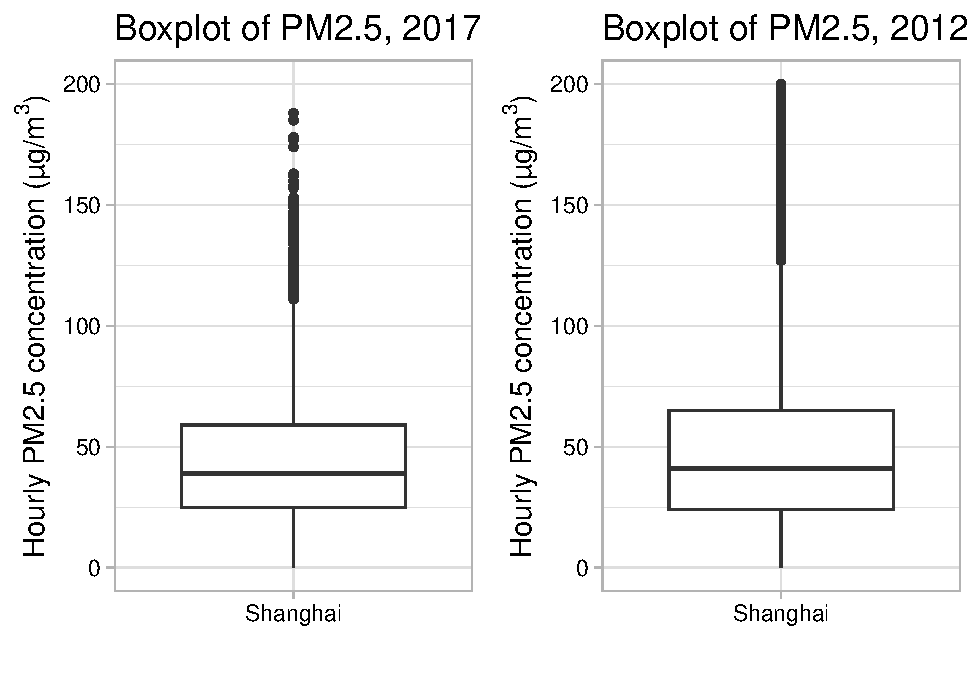
\includegraphics{Project_Template_files/figure-latex/Exploratory graph 3-1.pdf}
\caption{Boxplot of PM2.5 concentration in Shanghai, 2017 and 2012}
\end{figure}

\emph{Figure 3 Compares the mean PM2.5 concentrations of 2012 and 2017}

\begin{Shaded}
\begin{Highlighting}[]
\CommentTok{#combine Shanghai data into one dataframe}
\NormalTok{Shanghai12to17 <-}\StringTok{ }\KeywordTok{do.call}\NormalTok{(}\StringTok{"rbind"}\NormalTok{, }\KeywordTok{list}\NormalTok{(shanghai_}\DecValTok{2012}\NormalTok{, shanghai_}\DecValTok{2013}\NormalTok{, shanghai_}\DecValTok{2014}\NormalTok{, shanghai_}\DecValTok{2015}\NormalTok{, shanghai_}\DecValTok{2016}\NormalTok{, shanghai_}\DecValTok{2017}\NormalTok{))}

\CommentTok{#filter out missing values and calculate daily average PM2.5 concentration}
\NormalTok{Shanghai12to17_Processed <-}\StringTok{ }\NormalTok{Shanghai12to17 }\OperatorTok
\StringTok{  }\KeywordTok{filter}\NormalTok{(QC.Name }\OperatorTok{==}\StringTok{ "Valid"} \OperatorTok{&}\StringTok{ }\NormalTok{Value }\OperatorTok{>=}\DecValTok{0}\NormalTok{)}\OperatorTok
\StringTok{  }\KeywordTok{group_by}\NormalTok{(Year,Month, Day)}\OperatorTok
\StringTok{  }\KeywordTok{summarise}\NormalTok{(}\DataTypeTok{Daily_Mean_PM25 =} \KeywordTok{mean}\NormalTok{(Value))}

\CommentTok{#Create Date}
\NormalTok{  Shanghai12to17_Processed}\OperatorTok{$}\NormalTok{Date <-}\StringTok{ }\KeywordTok{as.Date}\NormalTok{(}\KeywordTok{with}\NormalTok{(Shanghai12to17_Processed, }\KeywordTok{paste}\NormalTok{(Year, Month, Day, }\DataTypeTok{sep=}\StringTok{"-"}\NormalTok{)), }\StringTok{"%Y-%m-%d"}\NormalTok{)}

\CommentTok{#Rearrange columns}
\NormalTok{  Shanghai12to17_Processed <-}\StringTok{ }\NormalTok{Shanghai12to17_Processed[,}\KeywordTok{c}\NormalTok{(}\DecValTok{5}\NormalTok{,}\DecValTok{1}\NormalTok{,}\DecValTok{2}\NormalTok{,}\DecValTok{3}\NormalTok{,}\DecValTok{4}\NormalTok{)]}
\end{Highlighting}
\end{Shaded}

\begin{Shaded}
\begin{Highlighting}[]
\CommentTok{#Assign coordinates to each site}
\NormalTok{Beijing_}\DecValTok{2017}\OperatorTok{$}\NormalTok{Latitude <-}\StringTok{ }\FloatTok{39.95}
\NormalTok{  Beijing_}\DecValTok{2017}\OperatorTok{$}\NormalTok{Longitude <-}\StringTok{ }\FloatTok{116.47}
  
\NormalTok{Chengdu_}\DecValTok{2017}\OperatorTok{$}\NormalTok{Latitude <-}\StringTok{ }\FloatTok{30.63}
\NormalTok{  Chengdu_}\DecValTok{2017}\OperatorTok{$}\NormalTok{Longitude <-}\StringTok{ }\FloatTok{104.07}
  
\NormalTok{Guangzhou_}\DecValTok{2017}\OperatorTok{$}\NormalTok{Latitude <-}\StringTok{ }\FloatTok{23.12}
\NormalTok{  Guangzhou_}\DecValTok{2017}\OperatorTok{$}\NormalTok{Longitude <-}\StringTok{ }\FloatTok{113.32}

\NormalTok{Shenyang_}\DecValTok{2017}\OperatorTok{$}\NormalTok{Latitude <-}\StringTok{ }\FloatTok{41.78}
\NormalTok{  Shenyang_}\DecValTok{2017}\OperatorTok{$}\NormalTok{Longitude <-}\FloatTok{123.42}

\NormalTok{shanghai_}\DecValTok{2017}\OperatorTok{$}\NormalTok{Latitude <-}\StringTok{ }\FloatTok{31.21}
\NormalTok{  shanghai_}\DecValTok{2017}\OperatorTok{$}\NormalTok{Longitude <-}\StringTok{ }\FloatTok{121.44}

\CommentTok{#Combine data for all sites into one dataframe  }
\NormalTok{All_Sites_}\DecValTok{2017}\NormalTok{ <-}\StringTok{ }\KeywordTok{do.call}\NormalTok{(}\StringTok{"rbind"}\NormalTok{, }\KeywordTok{list}\NormalTok{(shanghai_}\DecValTok{2017}\NormalTok{, Shenyang_}\DecValTok{2017}\NormalTok{, Guangzhou_}\DecValTok{2017}\NormalTok{, Chengdu_}\DecValTok{2017}\NormalTok{, Beijing_}\DecValTok{2017}\NormalTok{))}

\CommentTok{#Filter out missing value and calculate daily average PM2.5 concentrations}
\NormalTok{All_Sites_2017_Processed <-}\StringTok{ }\NormalTok{All_Sites_}\DecValTok{2017} \OperatorTok
\StringTok{  }\KeywordTok{filter}\NormalTok{(QC.Name }\OperatorTok{==}\StringTok{ "Valid"} \OperatorTok{&}\StringTok{ }\NormalTok{Value }\OperatorTok{>=}\DecValTok{0}\NormalTok{)}\OperatorTok
\StringTok{  }\KeywordTok{group_by}\NormalTok{(Site, Year, Month, Day, Latitude, Longitude)}\OperatorTok
\StringTok{  }\KeywordTok{summarise}\NormalTok{(}\DataTypeTok{Daily_Mean_PM25 =} \KeywordTok{mean}\NormalTok{(Value))}

\NormalTok{All_Sites_2017_avg <-}\StringTok{ }\NormalTok{All_Sites_2017_Processed }\OperatorTok
\StringTok{  }\KeywordTok{group_by}\NormalTok{(Site, Latitude, Longitude) }\OperatorTok
\StringTok{  }\KeywordTok{summarise}\NormalTok{(}\DataTypeTok{meanPM25 =} \KeywordTok{mean}\NormalTok{(Daily_Mean_PM25),}
            \DataTypeTok{maxPM25 =} \KeywordTok{max}\NormalTok{(Daily_Mean_PM25))}
\end{Highlighting}
\end{Shaded}

\begin{Shaded}
\begin{Highlighting}[]
\CommentTok{#Create a simplified function to convert PM2.5 concentration to AQI }
\NormalTok{Concentration_to_AQI <-}\StringTok{ }\ControlFlowTok{function}\NormalTok{(C)\{}
  \ControlFlowTok{if}\NormalTok{ (C }\OperatorTok{<=}\StringTok{ }\FloatTok{55.4}\NormalTok{)\{}
    \KeywordTok{as.integer}\NormalTok{((C}\OperatorTok{-}\FloatTok{35.5}\NormalTok{)}\OperatorTok{*}\NormalTok{(}\DecValTok{150}\OperatorTok{-}\DecValTok{101}\NormalTok{)}\OperatorTok{/}\NormalTok{(}\FloatTok{55.4}\OperatorTok{-}\FloatTok{35.5}\NormalTok{)}\OperatorTok{+}\DecValTok{101}\NormalTok{)}
\NormalTok{  \} }\ControlFlowTok{else}\NormalTok{\{}
    \ControlFlowTok{if}\NormalTok{ (C }\OperatorTok{<=}\StringTok{ }\FloatTok{150.4}\NormalTok{)\{}
      \KeywordTok{as.integer}\NormalTok{((C}\OperatorTok{-}\FloatTok{55.5}\NormalTok{)}\OperatorTok{*}\NormalTok{(}\DecValTok{200}\OperatorTok{-}\DecValTok{151}\NormalTok{)}\OperatorTok{/}\NormalTok{(}\FloatTok{150.4}\OperatorTok{-}\FloatTok{55.5}\NormalTok{)}\OperatorTok{+}\DecValTok{151}\NormalTok{)}
\NormalTok{    \}}
\NormalTok{  \}}
\NormalTok{\}}

\NormalTok{All_Sites_2017_avg <-}\StringTok{ }\KeywordTok{mutate}\NormalTok{(All_Sites_2017_avg, }\DataTypeTok{AQI =} \KeywordTok{Concentration_to_AQI}\NormalTok{(meanPM25))}
\end{Highlighting}
\end{Shaded}

\newpage

\section{Analysis}\label{analysis}

\begin{Shaded}
\begin{Highlighting}[]
\CommentTok{#run a Mann-Kendall test on the PM2.5 concentration in Shanghai from 2012 to 2017}
\KeywordTok{mk.test}\NormalTok{(Shanghai12to17_Processed}\OperatorTok{$}\NormalTok{Daily_Mean_PM25)}
\end{Highlighting}
\end{Shaded}

\begin{verbatim}
## 
##  Mann-Kendall trend test
## 
## data:  Shanghai12to17_Processed$Daily_Mean_PM25
## z = -4.6494, n = 1995, p-value = 3.329e-06
## alternative hypothesis: true S is not equal to 0
## sample estimates:
##             S          varS           tau 
## -1.381510e+05  8.829007e+08 -6.947051e-02
\end{verbatim}

\begin{Shaded}
\begin{Highlighting}[]
\CommentTok{#Run a Pettitt's Test to check if there are changing points}
\KeywordTok{pettitt.test}\NormalTok{(Shanghai12to17_Processed}\OperatorTok{$}\NormalTok{Daily_Mean_PM25)}
\end{Highlighting}
\end{Shaded}

\begin{verbatim}
## 
##  Pettitt's test for single change-point detection
## 
## data:  Shanghai12to17_Processed$Daily_Mean_PM25
## U* = 145860, p-value = 2.103e-07
## alternative hypothesis: two.sided
## sample estimates:
## probable change point at time K 
##                            1597
\end{verbatim}

\begin{Shaded}
\begin{Highlighting}[]
\KeywordTok{mk.test}\NormalTok{(Shanghai12to17_Processed}\OperatorTok{$}\NormalTok{Daily_Mean_PM25[}\DecValTok{1}\OperatorTok{:}\DecValTok{1597}\NormalTok{])}
\end{Highlighting}
\end{Shaded}

\begin{verbatim}
## 
##  Mann-Kendall trend test
## 
## data:  Shanghai12to17_Processed$Daily_Mean_PM25[1:1597]
## z = -0.1021, n = 1597, p-value = 0.9187
## alternative hypothesis: true S is not equal to 0
## sample estimates:
##            S         varS          tau 
## -2.17400e+03  4.52980e+08 -1.70621e-03
\end{verbatim}

\begin{Shaded}
\begin{Highlighting}[]
\KeywordTok{mk.test}\NormalTok{(Shanghai12to17_Processed}\OperatorTok{$}\NormalTok{Daily_Mean_PM25[}\DecValTok{1598}\OperatorTok{:}\DecValTok{1995}\NormalTok{])}
\end{Highlighting}
\end{Shaded}

\begin{verbatim}
## 
##  Mann-Kendall trend test
## 
## data:  Shanghai12to17_Processed$Daily_Mean_PM25[1598:1995]
## z = 3.7256, n = 398, p-value = 0.0001948
## alternative hypothesis: true S is not equal to 0
## sample estimates:
##            S         varS          tau 
## 9.880000e+03 7.031225e+06 1.250910e-01
\end{verbatim}

\begin{Shaded}
\begin{Highlighting}[]
\CommentTok{# Is there a second change point?}
\KeywordTok{pettitt.test}\NormalTok{(Shanghai12to17_Processed}\OperatorTok{$}\NormalTok{Daily_Mean_PM25[}\DecValTok{1598}\OperatorTok{:}\DecValTok{1995}\NormalTok{])}
\end{Highlighting}
\end{Shaded}

\begin{verbatim}
## 
##  Pettitt's test for single change-point detection
## 
## data:  Shanghai12to17_Processed$Daily_Mean_PM25[1598:1995]
## U* = 19508, p-value = 4.084e-16
## alternative hypothesis: two.sided
## sample estimates:
## probable change point at time K 
##                             158
\end{verbatim}

\begin{Shaded}
\begin{Highlighting}[]
\CommentTok{# Run another Mann-Kendall for the second change point}
\KeywordTok{mk.test}\NormalTok{(Shanghai12to17_Processed}\OperatorTok{$}\NormalTok{Daily_Mean_PM25[}\DecValTok{1598}\OperatorTok{:}\DecValTok{1755}\NormalTok{])}
\end{Highlighting}
\end{Shaded}

\begin{verbatim}
## 
##  Mann-Kendall trend test
## 
## data:  Shanghai12to17_Processed$Daily_Mean_PM25[1598:1755]
## z = -4.5497, n = 158, p-value = 5.373e-06
## alternative hypothesis: true S is not equal to 0
## sample estimates:
##             S          varS           tau 
## -3.027000e+03  4.423650e+05 -2.441326e-01
\end{verbatim}

\begin{Shaded}
\begin{Highlighting}[]
\KeywordTok{mk.test}\NormalTok{(Shanghai12to17_Processed}\OperatorTok{$}\NormalTok{Daily_Mean_PM25[}\DecValTok{1756}\OperatorTok{:}\DecValTok{1995}\NormalTok{])}
\end{Highlighting}
\end{Shaded}

\begin{verbatim}
## 
##  Mann-Kendall trend test
## 
## data:  Shanghai12to17_Processed$Daily_Mean_PM25[1756:1995]
## z = -5.3089, n = 240, p-value = 1.103e-07
## alternative hypothesis: true S is not equal to 0
## sample estimates:
##             S          varS           tau 
## -6.601000e+03  1.545518e+06 -2.302206e-01
\end{verbatim}

\begin{Shaded}
\begin{Highlighting}[]
\KeywordTok{pettitt.test}\NormalTok{(Shanghai12to17_Processed}\OperatorTok{$}\NormalTok{Daily_Mean_PM25[}\DecValTok{1598}\OperatorTok{:}\DecValTok{1755}\NormalTok{])}
\end{Highlighting}
\end{Shaded}

\begin{verbatim}
## 
##  Pettitt's test for single change-point detection
## 
## data:  Shanghai12to17_Processed$Daily_Mean_PM25[1598:1755]
## U* = 3356, p-value = 8.076e-08
## alternative hypothesis: two.sided
## sample estimates:
## probable change point at time K 
##                              65
\end{verbatim}

\begin{Shaded}
\begin{Highlighting}[]
\KeywordTok{mk.test}\NormalTok{(Shanghai12to17_Processed}\OperatorTok{$}\NormalTok{Daily_Mean_PM25[}\DecValTok{1598}\OperatorTok{:}\DecValTok{1662}\NormalTok{])}
\end{Highlighting}
\end{Shaded}

\begin{verbatim}
## 
##  Mann-Kendall trend test
## 
## data:  Shanghai12to17_Processed$Daily_Mean_PM25[1598:1662]
## z = 0.40196, n = 65, p-value = 0.6877
## alternative hypothesis: true S is not equal to 0
## sample estimates:
##            S         varS          tau 
## 7.200000e+01 3.120000e+04 3.461538e-02
\end{verbatim}

\begin{Shaded}
\begin{Highlighting}[]
\KeywordTok{mk.test}\NormalTok{(Shanghai12to17_Processed}\OperatorTok{$}\NormalTok{Daily_Mean_PM25[}\DecValTok{1663}\OperatorTok{:}\DecValTok{1755}\NormalTok{])}
\end{Highlighting}
\end{Shaded}

\begin{verbatim}
## 
##  Mann-Kendall trend test
## 
## data:  Shanghai12to17_Processed$Daily_Mean_PM25[1663:1755]
## z = 0.84963, n = 93, p-value = 0.3955
## alternative hypothesis: true S is not equal to 0
## sample estimates:
##            S         varS          tau 
## 2.570000e+02 9.078567e+04 6.009588e-02
\end{verbatim}

\begin{Shaded}
\begin{Highlighting}[]
\KeywordTok{pettitt.test}\NormalTok{(Shanghai12to17_Processed}\OperatorTok{$}\NormalTok{Daily_Mean_PM25[}\DecValTok{1756}\OperatorTok{:}\DecValTok{1995}\NormalTok{])}
\end{Highlighting}
\end{Shaded}

\begin{verbatim}
## 
##  Pettitt's test for single change-point detection
## 
## data:  Shanghai12to17_Processed$Daily_Mean_PM25[1756:1995]
## U* = 6169, p-value = 1.436e-07
## alternative hypothesis: two.sided
## sample estimates:
## probable change point at time K 
##                             170
\end{verbatim}

\begin{Shaded}
\begin{Highlighting}[]
\KeywordTok{mk.test}\NormalTok{(Shanghai12to17_Processed}\OperatorTok{$}\NormalTok{Daily_Mean_PM25[}\DecValTok{1756}\OperatorTok{:}\DecValTok{1925}\NormalTok{])}
\end{Highlighting}
\end{Shaded}

\begin{verbatim}
## 
##  Mann-Kendall trend test
## 
## data:  Shanghai12to17_Processed$Daily_Mean_PM25[1756:1925]
## z = 0.014824, n = 170, p-value = 0.9882
## alternative hypothesis: true S is not equal to 0
## sample estimates:
##            S         varS          tau 
## 1.200000e+01 5.506513e+05 8.355673e-04
\end{verbatim}

\begin{Shaded}
\begin{Highlighting}[]
\KeywordTok{mk.test}\NormalTok{(Shanghai12to17_Processed}\OperatorTok{$}\NormalTok{Daily_Mean_PM25[}\DecValTok{1926}\OperatorTok{:}\DecValTok{1995}\NormalTok{])}
\end{Highlighting}
\end{Shaded}

\begin{verbatim}
## 
##  Mann-Kendall trend test
## 
## data:  Shanghai12to17_Processed$Daily_Mean_PM25[1926:1995]
## z = -2.2459, n = 70, p-value = 0.02471
## alternative hypothesis: true S is not equal to 0
## sample estimates:
##             S          varS           tau 
##  -444.0000000 38905.3333333    -0.1839652
\end{verbatim}

\emph{According to the first Mann-Kendall Test, p-value \textless{}
0.0001, S = -1.38e+05 so there is a decreasing trend in PM2.5
concentrations in Shanghai from 2012 to 2017}

\begin{Shaded}
\begin{Highlighting}[]
\NormalTok{Shanghai12to17_Monthly <-}\StringTok{ }\NormalTok{Shanghai12to17_Processed }\OperatorTok
\StringTok{  }\KeywordTok{group_by}\NormalTok{(Year,Month)}\OperatorTok
\StringTok{  }\KeywordTok{summarise}\NormalTok{(}\DataTypeTok{Monthly_Mean_PM25 =} \KeywordTok{mean}\NormalTok{(Daily_Mean_PM25))}

\NormalTok{Shanghai12to17_Monthly}\OperatorTok{$}\NormalTok{Date <-}\StringTok{ }\KeywordTok{as.Date}\NormalTok{(}\KeywordTok{with}\NormalTok{(Shanghai12to17_Monthly, }\KeywordTok{paste}\NormalTok{(Year, Month,}\StringTok{"01"}\NormalTok{, }\DataTypeTok{sep=}\StringTok{"-"}\NormalTok{)), }\StringTok{"%Y-%m-%d"}\NormalTok{)}

\CommentTok{# Create a time series object}
\NormalTok{Shanghai12to17_timeseries <-}\StringTok{ }\KeywordTok{ts}\NormalTok{(Shanghai12to17_Monthly}\OperatorTok{$}\NormalTok{Monthly_Mean_PM25, }
                                \DataTypeTok{start =} \KeywordTok{c}\NormalTok{(}\DecValTok{2012}\NormalTok{, }\DecValTok{1}\NormalTok{) ,}\DataTypeTok{frequency =} \DecValTok{12}\NormalTok{)}
\NormalTok{Shanghai12to17_timeseries}
\end{Highlighting}
\end{Shaded}

\begin{verbatim}
##            Jan       Feb       Mar       Apr       May       Jun       Jul
## 2012  64.39169  53.10445  67.14090  54.95019  55.70430  40.16078  26.55297
## 2013 101.46242  64.25839  64.96774  61.61860  53.23069  44.33886  32.14922
## 2014  72.61396  52.32508  54.39317  51.65912  61.19360  42.12621  35.17865
## 2015  84.64382  66.46796  50.98786  52.40304  40.98860  36.55009  35.35663
## 2016  72.58816  57.58583  55.78133  56.02394  48.52583  35.32621  34.72419
## 2017  52.58442  56.67838  51.04167  49.21948  32.92391  30.73789          
##            Aug       Sep       Oct       Nov       Dec
## 2012  16.12474  44.06365  55.51799  67.04937  64.37512
## 2013  26.45089  27.97110  36.20997  79.18295 122.15358
## 2014  29.41896  29.09568  38.79696  53.27199  74.75655
## 2015  35.41667  28.07370  38.43414  55.90320  82.21746
## 2016  20.21237  28.34902  20.96657  50.00350  64.36563
## 2017
\end{verbatim}

\begin{Shaded}
\begin{Highlighting}[]
\CommentTok{# Run a Seasonal Mann-Kendall test}
\NormalTok{Shanghai.smktest <-}\StringTok{ }\KeywordTok{smk.test}\NormalTok{(Shanghai12to17_timeseries)}
\NormalTok{Shanghai.smktest}
\end{Highlighting}
\end{Shaded}

\begin{verbatim}
## 
##  Seasonal Mann-Kendall trend test (Hirsch-Slack test)
## 
## data:  Shanghai12to17_timeseries
## z = -2.6169, p-value = 0.008873
## alternative hypothesis: true S is not equal to 0
## sample estimates:
##    S varS 
##  -44  270
\end{verbatim}

\begin{Shaded}
\begin{Highlighting}[]
\KeywordTok{summary}\NormalTok{(Shanghai.smktest)}
\end{Highlighting}
\end{Shaded}

\begin{verbatim}
## 
##  Seasonal Mann-Kendall trend test (Hirsch-Slack test)
## 
## data: Shanghai12to17_timeseries
## alternative hypothesis: two.sided
## 
## Statistics for individual seasons
## 
## H0
##                      S varS    tau      z Pr(>|z|)  
## Season 1:   S = 0   -5 28.3 -0.333 -0.751 0.452370  
## Season 2:   S = 0    1 28.3  0.067  0.000 1.000000  
## Season 3:   S = 0   -9 28.3 -0.600 -1.503 0.132855  
## Season 4:   S = 0   -5 28.3 -0.333 -0.751 0.452370  
## Season 5:   S = 0   -9 28.3 -0.600 -1.503 0.132855  
## Season 6:   S = 0  -11 28.3 -0.733 -1.879 0.060289 .
## Season 7:   S = 0    6 16.7  0.600  1.225 0.220671  
## Season 8:   S = 0    4 16.7  0.400  0.735 0.462433  
## Season 9:   S = 0   -2 16.7 -0.200 -0.245 0.806496  
## Season 10:   S = 0  -6 16.7 -0.600 -1.225 0.220671  
## Season 11:   S = 0  -6 16.7 -0.600 -1.225 0.220671  
## Season 12:   S = 0  -2 16.7 -0.200 -0.245 0.806496  
## ---
## Signif. codes:  0 '***' 0.001 '**' 0.01 '*' 0.05 '.' 0.1 ' ' 1
\end{verbatim}

\begin{Shaded}
\begin{Highlighting}[]
\CommentTok{#See if there is a change point.}
\KeywordTok{pettitt.test}\NormalTok{(Shanghai12to17_timeseries)}
\end{Highlighting}
\end{Shaded}

\begin{verbatim}
## 
##  Pettitt's test for single change-point detection
## 
## data:  Shanghai12to17_timeseries
## U* = 296, p-value = 0.3302
## alternative hypothesis: two.sided
## sample estimates:
## probable change point at time K 
##                              52
\end{verbatim}

\begin{figure}
\centering
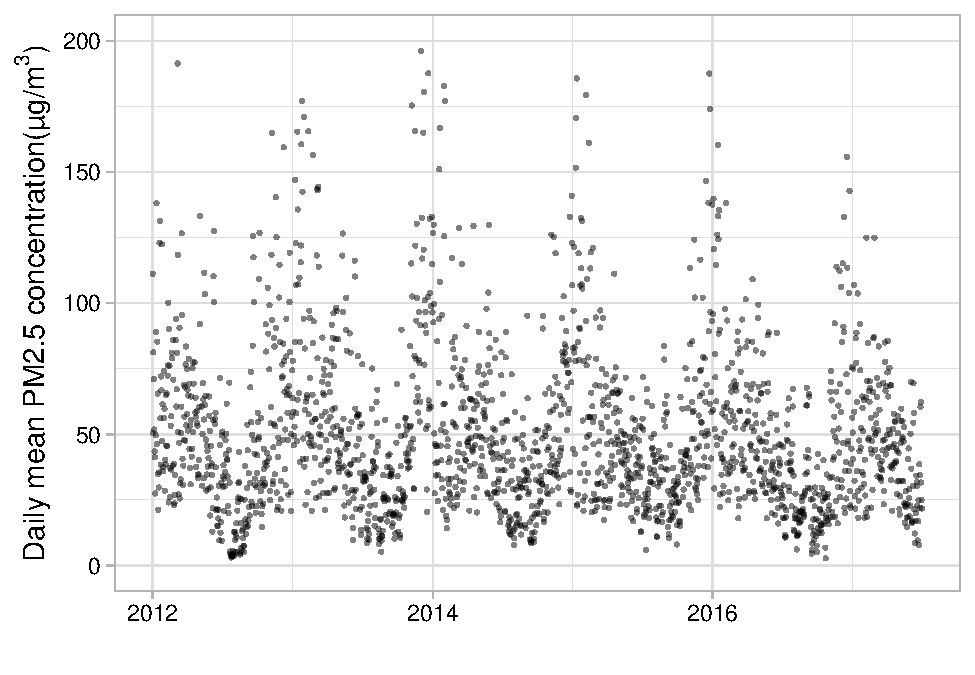
\includegraphics{Project_Template_files/figure-latex/unnamed-chunk-2-1.pdf}
\caption{Initial visualization of Shanghai PM2.5 concentration from 2012
to 2017}
\end{figure}

\begin{figure}
\centering
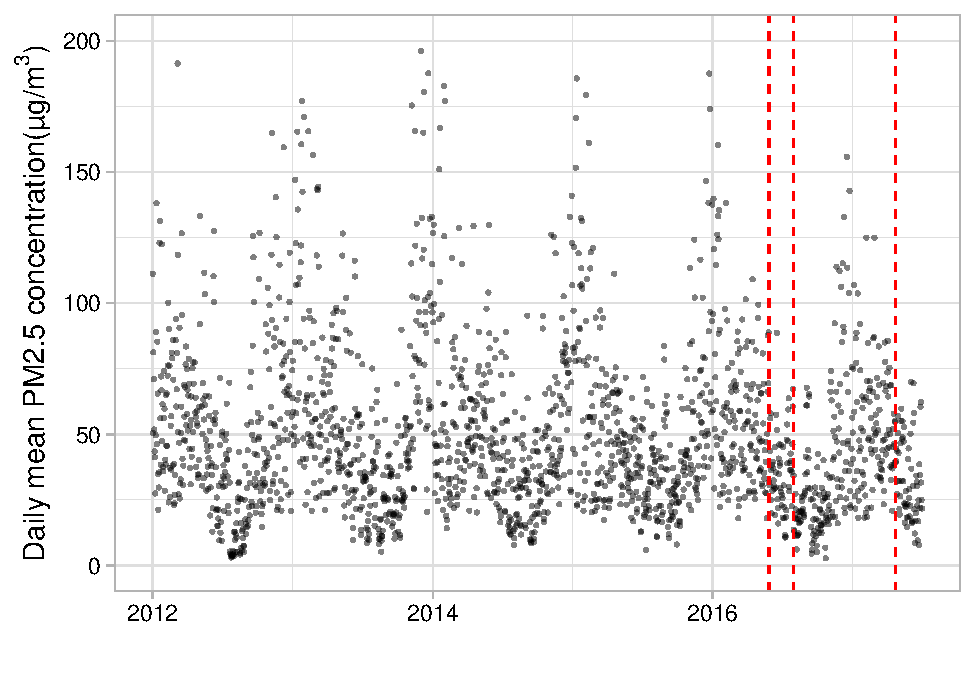
\includegraphics{Project_Template_files/figure-latex/unnamed-chunk-3-1.pdf}
\caption{Shanghai PM2.5 concentration from 2012 to 2017 with changing
points}
\end{figure}

\begin{figure}
\centering
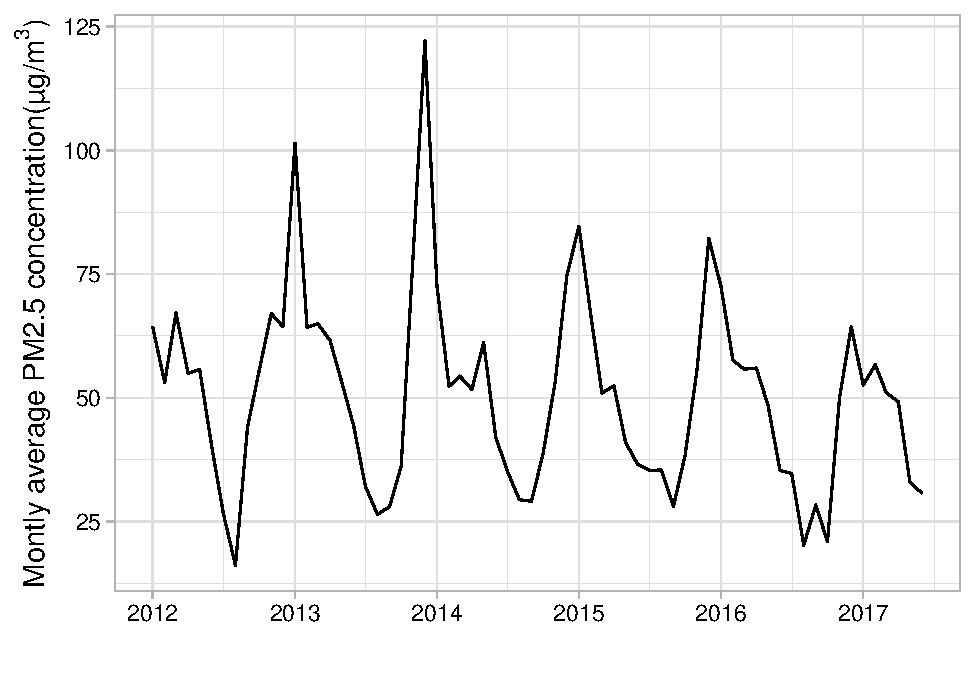
\includegraphics{Project_Template_files/figure-latex/unnamed-chunk-4-1.pdf}
\caption{Shanghai Monthly average PM2.5 concentration from 2012 to 2017}
\end{figure}

\begin{figure}
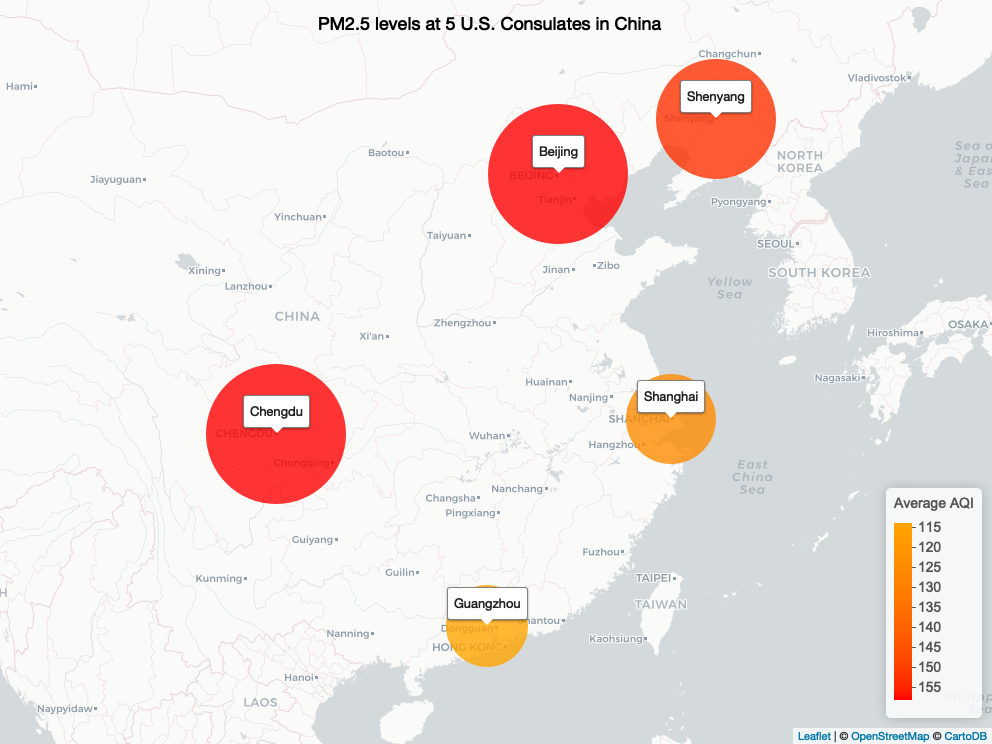
\includegraphics[width=1\linewidth]{myMap} \caption{PM2.5 levels at 5 U.S. Consulates in China}\label{fig:PM2.5 levels at 5 U.S. Consulates in China}
\end{figure}

\emph{The changing points in figure 5 seem to be due to the seasonal
variations, so I decide to look at the monthly variation of PM2.5
concentration to see if there exists seasonality}

\emph{Figure 6 shows that the PM2.5 concentraions do vary a lot over
months. Generally the concentrations peak in Winter and reach lowest in
Summer. Therefore, I decide to run a Seasonal Mann-Kendall test to
reduce to effect of seasonal trends that obscure the overall direction
of the trend}

\emph{Figure 7 shows the average PM2.5 concentration in 5 cities in
China in 2017. The larger the circle, the higher the concentration. In
the HTML format, the exact AQI value will pop up if the circle is
clicked, but this function is not available in the PDF format.} \newpage

\section{Summary and Conclusions}\label{summary-and-conclusions}

Pronounced seasonal variation is observed in PM2.5 concentrations in
Shanghai, with the highest concentrations typically observed in the
winter and the lowest concentrations generally found in the summer. From
2012 to 2017, there existed a decreasing trend in PM2.5 concentrations
in Shanghai(Seasonal Mann-Kendall test, p-value = 0.008873, S = -44).
China's government has made some progress to improve air quality.
However, the 2017 average AQI in Shanghai was 125, which falls into the
``unhealthy for sensitive groups'' range.

As for other 4 cities, Beijing and Chengdu showed highest PM2.5
concentration in 2017, with the AQI level reaching 158. Guangzhou showed
lowest AQI in 2017, which is 114; the 2017 average AQI in Shenyang was
153, also within the unhealthy range. Transportation and Coal combustion
are two major sources of PM2.5 in China. Transportation contributes a
lot to the PM2.5 concentration in Beijing and Chengdu. These two cities
rank first and second in terms of car ownership in China.


\end{document}
